% -------------------------------------
%               Setup
% -------------------------------------
\documentclass[t,24pt]{beamer}
\usepackage{lipsum}
\usepackage{KUstyle}
\toplinje{Meeting | Week 2} % The text at top. Remove the command if no text is desired

% -------------------------------------
% Command with question slides counter
% -------------------------------------
\newcounter{currentQSlide}
\newcounter{totalQSlide}

\newcommand{\resetsubject}{%
    \setcounter{currentQSlide}{0}
}

\setcounter{totalQSlide}{5}

\resetsubject

\newcommand{\incrementQSlideCnt}{%
    \stepcounter{currentQSlide}
}

% -------------------------------------
%                TiKz
% -------------------------------------

\usepackage{tikz}
\usetikzlibrary{shapes.geometric, arrows}

\tikzstyle{startstop} = [rectangle, rounded corners, minimum width=3.5cm, minimum height=1cm, text centered, draw=black, fill=blue!20]
\tikzstyle{process} = [rectangle, minimum width=3.5cm, minimum height=1cm, text centered, draw=black, fill=green!20]
\tikzstyle{arrow} = [thick,->,>=stealth]

\begin{document}
% The first slide. One can for instance change the main title, the subtitle, speaker, KU-unit and date
{
\setbeamertemplate{background}{
\includegraphics[width=\paperwidth,height=\paperheight]{KU/forside.pdf}}
\begin{frame}
    \begin{textblock*}{\textwidth}(0\textwidth,0.1\textheight)
        \begin{beamercolorbox}[wd=6.3cm,ht=7.7cm,sep=0.5cm]{hvidbox}
            \fontsize{4}{10}\fontfamily{ptm}\selectfont \textls[200]{UNIVERSITY OF COPENHAGEN}
            \noindent\textcolor{KUrod}{\rule{5.3cm}{0.4pt}}
        \end{beamercolorbox}
    \end{textblock*}
    \begin{textblock*}{\textwidth}(0\textwidth,0.1\textheight)
        \begin{beamercolorbox}[wd=6.3cm,sep=0.5cm]{hvidbox}
                \Large \textcolor{KUrod}{Meeting - Week 2}
                \vspace{0.5cm}
                \par
                \large Progress, Challenges \& Next steps
                \vspace{0.5cm}
                \par
                \textcolor{gray}{\scriptsize Simon Winther \& Hjalte Bjoernstrup, Department of Computer Science, University of Copenhagen (DIKU), \today.}
        \end{beamercolorbox}
    \end{textblock*}
    \begin{textblock}{1}(6,11.44)
        
\includegraphics[width=1cm]{KU/KU-logo.png}
    \end{textblock}
\end{frame}
}
% ----------------------------------------------------
%                       Slide 1
% ----------------------------------------------------
\begin{frame}[hoved]
\incrementQSlideCnt
\frametitle{Questions? (\thecurrentQSlide/\thetotalQSlide)}
\begin{enumerate}
\item Is it permitted to stream while coding on platforms like Twitch or YouTube, not for providing help, but simply because it’s fun and motivating to stream while working on a project?
\item Are we allowed to install missing PIP libraries, such as Hydra and other modules, if they are not found in the local environment, or should we ask for permission before doing so?
\item Are we allowed to use Docker? We attempted to use it, but it required the sudo command, which we are not allowed to use. Would it be possible to be added as Docker users, or is there another way to run it without sudo? Also, do we need to use Docker for the UNET 3+, and if so, does it impact performance (e.g., making it slower), or is it fine?

\end{enumerate}
\end{frame}

% ----------------------------------------------------
%                       Slide 2
% ----------------------------------------------------

\begin{frame}[hoved]
\incrementQSlideCnt
\frametitle{Questions? (\thecurrentQSlide/\thetotalQSlide)}
\begin{enumerate}
\setcounter{enumi}{3}
\item Are we allowed to use multiple GPUs for training? Specifically, if we notice that two GPUs are currently inactive or idle, can we use them for training the model? Or would you prefer that we always use only a single GPU?
\item We noticed that many papers had excellent modeling and visualizations of CNN and U-Net architectures. We were wondering which tools you and other authors used to create these high-quality figures so that we could generate similar ones ourselves.
\end{enumerate}
\end{frame}

% ----------------------------------------------------
%                       Slide 3
% ----------------------------------------------------

\begin{frame}{Model Progression}
    \begin{columns}
        \column{0.45\textwidth}
        \textbf{Model Hierarchy}
        
        \vspace{0.5cm}
        To the right, you can see a figure illustrating our proposed model progression, to ensure that it aligns with what we talked about in the last meeting.
        \begin{itemize}
            \item U-Net
            \item MS U-Net
            \item 3D DiffNet
            \item MS 3D DiffNet
        \end{itemize}

        \column{0.45\textwidth}
        \vspace{-1.5cm}
        \begin{figure}
            \centering
            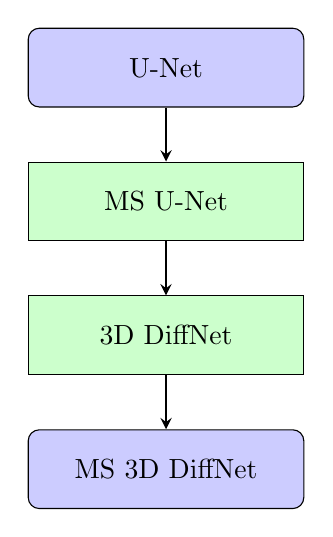
\begin{tikzpicture}[node distance=1.7cm]
                % Nodes
                \node (unet) [startstop] {U-Net};
                \node (msunet) [process, below of=unet] {MS U-Net};
                \node (diff3D) [process, below of=msunet] {3D DiffNet};
                \node (ms3Ddiff) [startstop, below of=diff3D] {MS 3D DiffNet};
        
                % Arrows
                \draw [arrow] (unet) -- (msunet);
                \draw [arrow] (msunet) -- (diff3D);
                \draw [arrow] (diff3D) -- (ms3Ddiff);
            \end{tikzpicture}
            \caption{Model progression from U-Net to MS 3D DiffNet}
            \label{fig:model_progression}
        \end{figure}
    \end{columns}
\end{frame}

% ----------------------------------------------------
%                       Slide 4
% ----------------------------------------------------
\begin{frame}[hoved]
\incrementQSlideCnt
\frametitle{Questions? (\thecurrentQSlide/\thetotalQSlide)}
\begin{enumerate}
\setcounter{enumi}{5}
\item \small So, we wanted to ask whether the proposed model progression aligns with what we discussed in our last meeting as mentioned already.
\item \small After successfully training the U-Net 3+ model, should we evaluate that one first—storing its performance, using validation/testing data, and checking metrics like score or log-likelihood—before proceeding to train other models, or should we take a different approach?
\item \small Would it be possible to get an overview of the project timeline for the next few weeks? This would help us structure our focus areas. If this isn’t something that can be provided, that’s completely fine. We were simply just curious.
\item We find that papers formatted in two columns look very professional, and we wanted to ask if it would be acceptable to use this format for our paper, or if it would be a bad idea and something we should avoid.

\end{enumerate}
\end{frame}

% ----------------------------------------------------
%                       Slide 5
% ----------------------------------------------------
\begin{frame}[hoved]
\incrementQSlideCnt
\frametitle{Questions? (\thecurrentQSlide/\thetotalQSlide)}
\begin{enumerate}
\setcounter{enumi}{10}
\item When do you think we should start writing the paper, and what key aspects should we include? Would it be relevant to present the architectures of the multi-scale U-Net 3+ and the multi-scale 3D Diffusion Network, similar to how other papers illustrate model architectures? Should we also cover the mathematical foundations of diffusion models, or what would you recommend we focus on?
\item Since we haven't been able to run the training yet, we're unsure if there’s already a built-in tool for visualizing and storing training progress—something like Weights \& Biases, where you can track loss and other metrics. If such a system isn't included, would it be okay for us to integrate a library like Weights \& Biases and add logging to track the training process?
\end{enumerate}
\end{frame}


% ----------------------------------------------------
%                       Slide 5
% ----------------------------------------------------
\begin{frame}[hoved]
\incrementQSlideCnt
\frametitle{Questions? (\thecurrentQSlide/\thetotalQSlide)}
\begin{enumerate}
\setcounter{enumi}{13}
\item \small Just to confirm, we only need to modify the code for three models. First, we clone the U-Net 3+ repository, train it as is, and store its performance in a table—this serves as the baseline U-Net 3+ model. At this point, no code changes are made; we simply run the model and record its accuracy. Next, we modify U-Net 3+ by adding multi-scaling, train it, and store the performance results to compare it with the baseline. Then, we clone the DiffNet repository, modify it from 2D to 3D, train it, and store its performance—this serves as the 3D DiffNet baseline. Finally, we take the 3D DiffNet and add multi-scaling, train it, and record its performance as well. In total, we will have four models in our comparison, but only three require actual code modifications: adding multi-scaling to U-Net 3+, converting DiffNet to 3D, and adding multi-scaling to the 3D DiffNet. Have we interpreted this correctly, or is there something we misunderstood?

\end{enumerate}
\end{frame}




\end{document}
